\subsection{Desenvolvimento de um Jogo para Auxílio no Ensino de Estruturas de Dados}

Durante o trabalho de conclusão de curso intitulado \textit{"Desenvolvimento de um Jogo para Auxílio no Ensino de Estruturas de Dados"}, foi desenvolvido um jogo digital mobile com o intuito de facilitar e auxiliar o ensino, a aprendizagem e a visualização dos conceitos de algoritmos de busca da disciplina de Estrutura de Dados. A tecnologia utilizada para desenvolver este jogo foi a linguagem de programação Dart, em conjunto com o framework Flutter. \cite{glatz2023desenvolvimento}

\begin{figure}[H]
	\centering
	\caption{Captura de tela do jogo para auxiliar em estrutura de dados}
	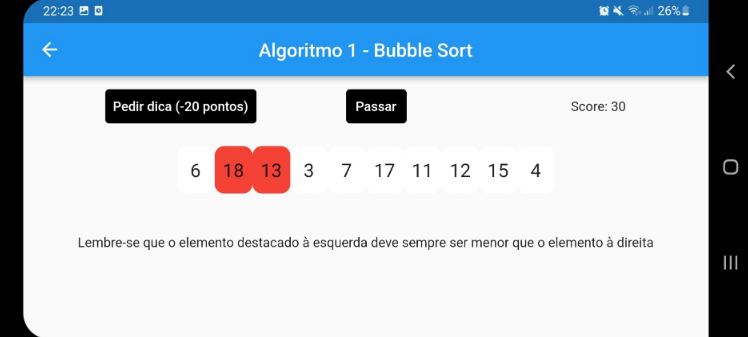
\includegraphics[width=0.8\textwidth]{images/aux-ed.png}
	\legend{Fonte: \cite{glatz2023desenvolvimento}}
	\label{fig:aux_ed}
\end{figure}


% TODO: ADD IMAGE

